\begin{frame}{Definición de Radiación}
  \textbf{Radiación:} Emisión y propagación de energía a través del
  espacio o de un medio material en forma de \alert{Ondas electromagnéticas} o
  \alert{Partículas subatómicas}.
  \vfill
  \begin{columns}[T]
    \begin{column}{0.48\textwidth}
      \begin{block}{Radiación Electromagnética}
        Energía en forma de ondas. Fotones.
        \begin{itemize}
          \item Luz visible
          \item Ondas de radio
          \item Rayos X
          \item Rayos gamma ($\gamma$)
        \end{itemize}
      \end{block}
    \end{column}

    \begin{column}{0.48\textwidth}
      \begin{block}{Radiación de Partículas}
        Partículas con masa y alta velocidad.
        \begin{itemize}
          \item Partículas alfa ($\alpha$)
          \item Partículas beta ($\beta$)
          \item Neutrones
          \item Protones
        \end{itemize}
      \end{block}
    \end{column}
  \end{columns}
  \vfill

  La radiación de alta energía es \alert{ionizante}: Suficiente energía
  para desligar electrones de los átomos, alterando la materia.
\end{frame}

\begin{frame}{Interacciones Electromagnéticas con la Materia}
  Diferentes regiones del espectro electromagnético, diferentes sus efectos e
  interacciones con la materia.

  Si \alert{fotones} penetran un medio material, existen dos mecanismos de
  atenuación:
  \begin{itemize}
    \item \textbf{Difusión:} El fotón es desviado, sin
      depositar energía en el medio.
    \item \textbf{Absorción:} El fotón transfiere energía a las partículas
      cargadas, causando ionización.
  \end{itemize}
\end{frame}

\begin{frame}{Ilustración interacción radiación-materia}
  \begin{figure}
    \centering
    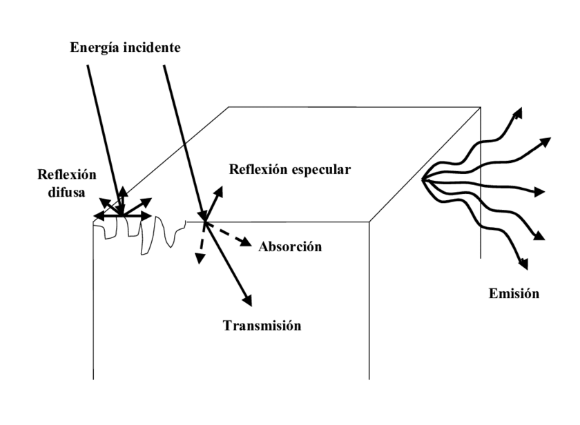
\includegraphics[width=0.6\linewidth]{../images/types_radiation.png}
    \caption{Representación de diferentes procesos ocurridos en la interacción radiación-materia.}
    \label{fig:types_radiation}
  \end{figure}
\end{frame}

\begin{frame}{Interacciones Electromagnéticas}
  El dominio de cada mecanismo depende de la energía del fotón ($E$) y del
  número atómico ($Z$) del material:

  \begin{itemize}
    \item \textbf{Efecto Fotoeléctrico:} Domina bajas energías.
    \item \textbf{Efecto Compton:} Domina a energías intermedias.
    \item \textbf{Producción de Pares:} Domina a energías altas ($>\qty{1.022}{
      \mega\eV}$).
  \end{itemize}
\end{frame}

\begin{frame}{Dominios de Interacción}
  \begin{figure}
    \centering
    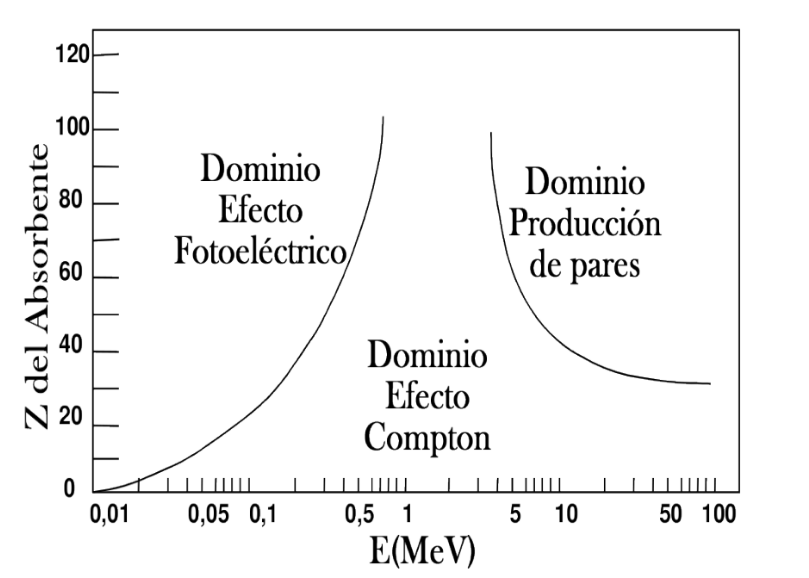
\includegraphics[width=0.6\linewidth]{../images/domains.png}
    \caption{Esquema de las regiones de dominio de los mecanismos de absorción
    de energía.}
    \label{fig:domains}
  \end{figure}
\end{frame}

\begin{frame}{Atenuación de fotones}
  La atenuación en un material homogéneo se describe por:
  \begin{block}{Ley de Beer-Lambert}
    $$I(x) = I_0 e^{-\mu x}$$
  \end{block}
  \begin{itemize}
    \item $I$ la intensidad tras pasar un grosor $x$.
    \item $I_0$ intensidad inicial.
    \item $\mu$ coeficiente de atenuación lineal.
  \end{itemize}

  El \alert{espesor medio} $x_{1/2} = \mu^{-1} \ln{2}$ y el \alert{coeficiente
  de atenuación} ${\rho}^{-1} \mu$ ($\rho$ densidad) son dependientes del
  material y la energía del fotón.
\end{frame}

\begin{frame}{Interacción con Partículas Cargadas}
  El paso de partículas cargadas a través de la materia se caracteriza por la
  pérdida de energía y la desviación de su trayectoria.

  \vfill
  \begin{block}{Tipos de Colisiones}
    \begin{itemize}
      \item \textbf{Con electrones atómicos:}
        \begin{itemize}
          \item \textit{Elástica}.
          \item \textit{Inelástica:} Ionización o excitación, con pérdida
            significativa de energía.
        \end{itemize}
      \item \textbf{Con núcleos atómicos:}
        \begin{itemize}
          \item \textit{Elástica}.
          \item \textit{Inelástica:} Frenado de la partícula y emisión de
            radiación (\textit{Bremsstrahlung}).
        \end{itemize}
    \end{itemize}
  \end{block}
\end{frame}

\begin{frame}{Esquema de las interacciones de partículas cargadas}
  \begin{figure}
    \centering
    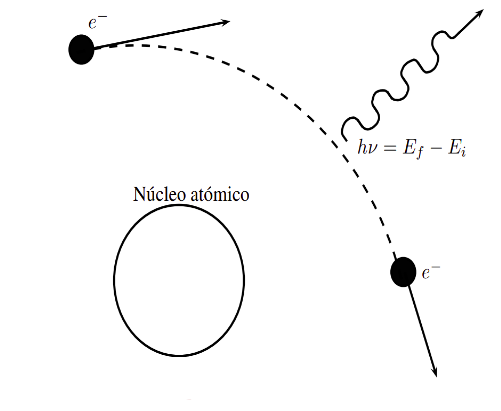
\includegraphics[width=0.55\linewidth]{../images/charged_particles.png}
    \caption{Proceso de Bremsstrahlung de un electrón de alta energía
    desviado por interacción de Coulomb del núcleo atómico.}
    \label{fig:charged_particles}
  \end{figure}
\end{frame}

\begin{frame}{Pérdida de Energía de Partículas Cargadas}
  \begin{itemize}
    \item \textbf{Por Ionización y Excitación (Fórmula de Bethe-Bloch):}
      \begin{equation*}
        -\frac{dE}{dx} = 4\pi
        r_{0}^{2}z^{2}\frac{m_{0}c^{2}}{\beta^{2}}N_{A}Z\left[\ln{\left(\frac{2m_{0}c^{2}}{I}\beta^{2}\gamma^{2}\right)}
        - \beta^{2}\right]
      \end{equation*}

    \item \textbf{Por Bremsstrahlung (Radiación de Frenado):}
      \begin{equation*}
        -\frac{dE}{dx} \approx 4\alpha N_{A}\frac{Z^{2}}{A}r_{0}^{2}E \ln{\frac{183}{Z^{1/3}}}
      \end{equation*}

    \item \textbf{Por Radiación Cherenkov:}
      \begin{itemize}
        \item Ocurre cuando una partícula viaja más rápido que la luz en ese medio.
        \item Es un mecanismo de pérdida de energía menos significativo.
      \end{itemize}
  \end{itemize}
\end{frame}

\begin{frame}{Pérdida de energía por partícula}
  \begin{figure}
    \centering
    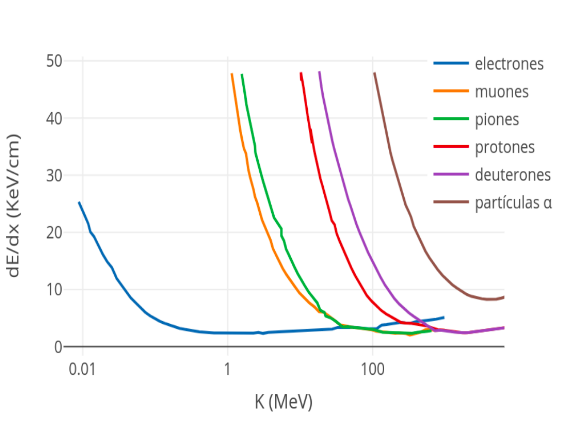
\includegraphics[width=0.6\linewidth]{../images/energy_loss.png}
    \caption{Pérdida de energía por unidad de recorrido en el plomo para
    diferentes partículas.}
    \label{fig:energy_loss}
  \end{figure}
\end{frame}

\begin{frame}{Interacciones de Neutrones}
  Los neutrones no tienen carga eléctrica, por lo que son una radiación
  \textbf{indirectamente ionizante}.

  \vfill
  \begin{block}{Proceso de Interacción}
    Interactúan mediante colisiones directas con los núcleos atómicos, generando
    partículas cargadas secundarias o fotones que sí ionizan el material.
  \end{block}

  \vfill
  Los mecanismos de interacción principales son:
  \begin{itemize}
    \item Dispersión elástica.
    \item Dispersión inelástica.
    \item Captura radiactiva.
    \item Fisión.
  \end{itemize}
\end{frame}
